% !TeX root = ../main.tex

\chapter{相关技术}

\section{AOSP project}

\subsection{Android通用内核}

Android 内核基于上游 Linux 长期支持 (LTS) 内核,google会在LTS内核的基础上结合安卓专用补丁,如bionic以及Ashmen等。
AOSP 通用内核(也称为 Android 通用内核或 ACK)是 kernel.org 内核的下游,包含与 Android 社区相关但尚未合并到 Mainline 
内核或长期支持 (LTS) 内核的补丁。这些补丁可能包括:
    Android 功能所需的向后移植和精选的上游功能
    可供 Android 设备使用但仍处于上游开发阶段的功能
    对其他生态合作伙伴有用的供应商/原始设备制造商 (OEM) 功能

android-mainline 是 Android 功能的主要开发分支。每当 Linus Torvalds 
发布内核版本或候选内核版本时,Linux Mainline 内核就会合并到 android-mainline 中。
在 2019 年之前,Android 通用内核是通过克隆最新声明的 LTS 内核并添加 Android 专用补丁程序来构建的。
2019 年,这一过程变成了从 android-mainline 中分支出新的 Android 通用内核。这种新模型以递增的方式构建内核,
从而避免进行大量的向前移植和测试 Android 补丁程序的工作。android-mainline 会经过大量持续不断的测试,
因此该模型可保证内核自发布之日起就具有很高的质量。

当上游声明新的 LTS 时,相应的通用内核就会从 android-mainline 分支出来。这样,合作伙伴就可以在上游声明 
LTS 版本之前,通过从 android-mainline 进行合并来开始项目。创建新的通用内核分支后,
合作伙伴可以将合并来源无缝更改为新的分支。
% 内核驱动是用于管理和控制图形处理单元的重要组件,允许操作系统和系统应用访问交互GPU硬件。

\subsection{AOSP开源安卓项目}
\subsubsection{Soong构建系统}

\begin{figure}[h]
  \centering
  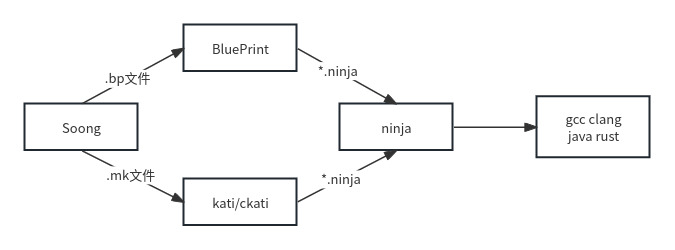
\includegraphics[width=0.8\textwidth]{soong结构示意图.jpg}
  \caption{Soong结构示意图}
\end{figure}

Soong 是 Android 构建系统的一部分,主要用于替代旧的 Makefile 系统。它是一个基于 Kati GNU Make 克隆工具和Ninja构建系统组件的构建工具,旨在简化和加速 Android 的构建过程。
相较于传统的Make 编译系统,Soong支持模块化和增量构建,并且支持并行处理多个构建任务,可以加快整体构建速度。简化了配置,相较于Android.mk文件,Android.bp文件更易读,并且可以
自动管理模块之间的依赖关系,减少了手动配置的需求。

在早期的Android版本中,编译系统主要依赖于 GNU Make。这个系统使用 Makefile 文件定义构建规则,适用于较小规模的项目。由于 Android 是一个庞大的操作系统,随着功能和组件的增加,
传统的 Makefile 系统逐渐显露出其缺乏模块化以及编译时间长等缺点。Makefile 适合较简单的构建过程,但在处理复杂的依赖关系时,效率较低,且不够灵活并且随着项目的扩大,编译时间显著增加,
影响了开发效率。

而为了解决这些问题,Google 在 Android 8.0(Oreo)中引入了 Soong 作为新的构建系统。Soong 的设计旨在解决 Makefile 的诸多不足,并提供更好的性能和可维护性。
基于 Blueprint 的构建:Soong 使用了一种名为 Blueprint 的配置语言,这种语言是针对 Android 特殊需求而设计的。Blueprint 使得定义模块及其依赖关系变得更加直观和灵活。
其具有高性能、模块化和可扩展性和集成 Gradle等多种优势。Soong 通过并行化构建过程和智能依赖分析,显著提高了编译速度,使得开发者能更快地迭代。
同时支持多种模块类型,包括 Java、C/C++ 和资源文件等,适应了 Android 多样化的构建需求。开发者可以通过编写新的 Blueprint 文件来扩展 Soong 的功能。
Soong 还与 Gradle 集成,为 Android 应用的构建提供了更好的支持,使得 Android 应用开发更加灵活和便捷。

\subsubsection{bionic}

Bionic 是 Android 操作系统中的 C 标准库,实现了 POSIX 兼容的功能。它是 Android 平台的核心组件之一,具有轻量、高效等特点,
满足移动设备的特定需求,并优化性能和资源使用。Bionic 的设计考虑了 Android 的多样性和复杂性,提供基础的系统调用和库函数,
为应用程序和系统服务提供了必要的底层支持。

Bionic 的开发始于 Android 项目的早期阶段,目的是为 Android 提供一个与 GNU C 库(glibc)兼容的替代品。随着 Android 的发展,Bionic 不断演进,
以适应移动设备的需求。它的设计初衷是为了减少内存占用,提高启动速度,并提供对 Android 特有功能的支持。
主要的特性有

1.轻量级:Bionic 的核心设计理念是轻量化。它去除了许多传统 C 库中的功能,专注于满足 Android 应用的实际需求。这使得 Bionic 
在资源受限的环境中表现出色。

2.性能优化:Bionic 针对移动设备进行了多项性能优化,包括内存管理和线程处理等。其快速的启动时间和低内存占用使得 
Android 应用能够更流畅地运行。

3.POSIX 兼容性:虽然 Bionic 不是完全的 POSIX 实现,但它提供了大部分 POSIX API,这使得从其他 Unix-like 
系统移植应用变得更加容易。

4.原生开发支持:Bionic 支持 Android 的原生开发工具(NDK),允许开发者在 C 和 C++ 中编写高性能代码。
这对于需要直接与硬件交互或执行计算密集型任务的应用尤为重要。

\subsection{Android图形协议}
Android 的图形协议是为移动设备特别设计的,包含了多个组件,如 SurfaceFlinger、Hardware Composer 
和各种图形库(如 OpenGL ES 和 Vulkan)。其设计理念主要体现在以下几个方面:

深度定制:Android 的图形协议针对移动设备的资源限制和性能要求进行了优化。它通过硬件加速和资源管理,
确保在低功耗和高性能之间取得平衡。

图形合成:SurfaceFlinger 作为 Android 的图形合成器,负责将多个图形层(如应用程序窗口、系统 UI 和视频内容)
合成到一起。这种设计允许流畅的动画和用户交互,提升了用户体验。

直接硬件访问:Android 的图形协议能够直接与硬件抽象层(HAL)交互,充分利用 GPU 的性能。
这使得 Android 在图形渲染方面能够实现高效处理,尤其是在游戏和多媒体应用中。

适应性强:针对各种不同的硬件平台,Android 的图形协议能够灵活适应,支持多种显示技术和分辨率。
这种适应性使其能够在不同的设备上提供一致的用户体验。

\begin{figure}[h]
  \centering
  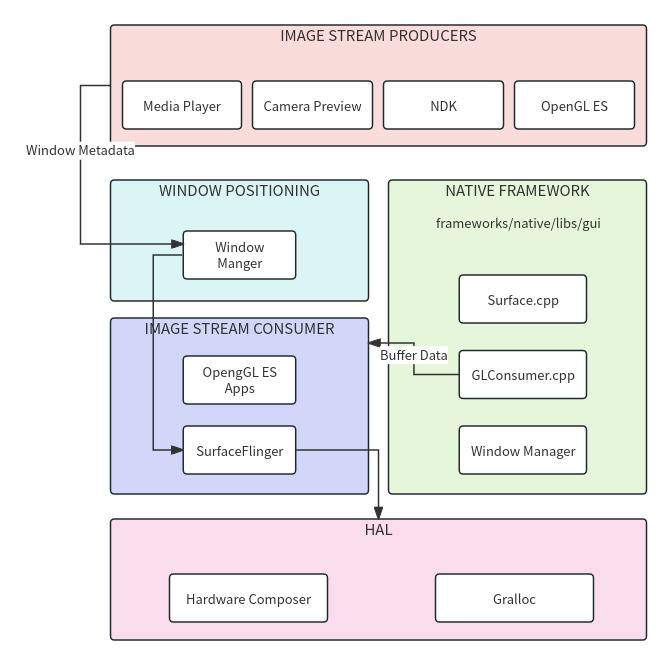
\includegraphics[width=0.8\textwidth]{安卓图形子系统架构图.jpg}
  \caption{安卓图形子系统架构图}
\end{figure}

\subsubsection{低级别组件}

1. BufferQueue 和 gralloc
BufferQueue 是一种机制,用于将生成图形数据的组件(生产者)连接到接受数据以进行显示或进一步处理的组件(消费者)。
它允许多个生产者和消费者之间高效地交换图形缓冲区。gralloc 是通过供应商专用 HAL 接口实现的内存分配器,
负责执行缓冲区的分配任务,为 BufferQueue 提供所需的图形缓冲区。这种设计使得内存管理更加灵活高效,
适用于 Android 生态系统中的各种图形需求。

2. SurfaceFlinger、Hardware Composer 和虚拟显示屏
SurfaceFlinger 是 Android 中的图形合成器,它接受来自多个源的数据缓冲区,并将它们合成成一个最终图像,然后发送到显示屏。
Hardware Composer HAL (HWC) 优化了这一过程,确定使用可用硬件合成缓冲区的最有效方法,以提高性能并减少 CPU 负担。虚拟显示屏 
则使合成输出可在系统内使用,支持如屏幕录制和通过网络发送屏幕内容等功能。

3. Surface、Canvas 和 SurfaceHolder
Surface 是一个可生成缓冲区队列的对象,通常由 SurfaceFlinger 使用。当渲染到 Surface 上时,
结果会出现在传送给消费者的缓冲区中。Canvas API 提供了一种软件绘图的方法,支持硬件加速,是 OpenGL ES 的低级替代方案。
所有与视图相关的操作都涉及到 SurfaceHolder,其 API 用于获取和设置 Surface 的参数,如大小和格式,从而为图形显示提供灵活性。

4. EGLSurface 和 OpenGL ES
OpenGL ES (GLES) 定义了一套图形渲染 API,旨在与 EGL 结合使用。EGL 是一个库,
负责创建和访问窗口,使得在操作系统上绘制图形成为可能。开发者使用 GLES 来绘制纹理多边形,
而通过 EGL 调用将渲染结果应用到屏幕上。EGL 还处理上下文管理和缓冲区交换,确保渲染的高效性与流畅性。

5. Vulkan
Vulkan 是一种高性能的 3D 图形 API,具有低开销和跨平台特性。与 OpenGL ES 相似,Vulkan 也提供创建高质量实时图形的工具,
但它在性能和灵活性上具备更大的优势。Vulkan 减少了 CPU 开销,使得开发者能够更直接地控制图形硬件。
此外,Vulkan 支持 SPIR-V 二进制中间语言,允许更加高效的着色器编译和执行,从而提升渲染性能和效率。

\subsubsection{高级别组件}

1. SurfaceView 和 GLSurfaceView
SurfaceView 是一种结合了 Surface 和 View 的组件。SurfaceView 的视图部分由 SurfaceFlinger 合成,
而不是由应用程序直接合成。这种设计允许在单独的线程或进程中进行渲染,使得 SurfaceView 与应用界面的渲染相互隔离,
从而提高了性能和响应性。GLSurfaceView 是 SurfaceView 的一个子类,专门用于 OpenGL ES 渲染。
它提供了管理 EGL 上下文、线程间通信以及与 Activity 生命周期交互的辅助功能,使得开发者能够更方便地进行 OpenGL ES 渲染,
尽管并不强制要求使用 GLES。

2. SurfaceTexture
SurfaceTexture 将 Surface 和 GLES 纹理结合在一起,创建了一个 BufferQueue。
应用程序充当这个 BufferQueue 的消费者。当生产者将新的缓冲区放入队列时,SurfaceTexture 会通知应用程序。
应用程序可以依次释放先前占用的缓冲区,从队列中获取新的缓冲区,并执行 EGL 调用,使 GLES 能够将此缓冲区作为外部纹理使用。
这种机制在 Android 7.0 中得到了增强,新增了对安全纹理视频播放的支持,允许对受保护的视频内容进行 GPU 后处理,
从而提升了视频播放的安全性和性能。

3. TextureView
TextureView 是一个结合了 View 和 SurfaceTexture 的组件。TextureView 封装了 SurfaceTexture,
负责处理回调以及获取新的缓冲区。在绘图时,TextureView 使用最近收到的缓冲区内容作为其数据源,
并根据 View 状态指示在需要渲染的位置和方式进行渲染。由于 View 合成始终通过 GLES 执行,
这意味着内容的更新可能导致其他 View 元素的重绘,从而确保了 UI 的一致性和动态性。


\section{龙芯平台支持}
\subsection{GPU硬件}
渲染管线、pipectrl
\subsection{固件}
来不及写了。。。
